
\section{Theorie}
\label{sec:Theorie}

\subsection{Das Franck-Hertz-Experiment}
Der Aufbau einer Franck-Hertz-Apparatur ist in Abbildung \ref{fig:apparat} zu sehen.
Beim Franck-Hertz-Versuch wird in einem evakuierten Gefäß ein Tropfen Quecksilber erhitzt, sodass es ausschließlich mit Hg-Dampf gefüllt ist. Der Sättigungsdampfdruck lässt sich dabei über die Temperatur $T$ regeln.
Durch eine Heizspannung wird eine in das Gefäß eingelassenen Glühkathode erhitzt, sodass Elektronen austreten. 
Das Gefäß wird durch ein Gitter in zwei Bereiche unterteilt:
Zwischen Kathode und Gitter herrscht eine Beschleunigungsspannung $U_.B$.
Es gilt für die kinetische Energie $E$ der Elektronen in diesem Bereich mit der Elektronenmasse $m_.e$ und der Elementarladung $e_.0$:
\begin{equation*}
E=\frac{m_.ev_.{vor^2}}{2}=e_.0U_.B
\end{equation*}
und damit für ihre Geschwindigkeit
\begin{equation*}
v_.{vor}=\sqrt{\frac{2e_.0U_.B}{m_.e}}
\end{equation*}
Da im gesamten Gefäß Hg-Dampf enthalten ist, kommt es auf dem Weg der Elektronen zu elastischen und inelastischen Stößen mit den Quecksilberatomen. Erstere treten aufgrund des Massenunterschieds zwischen Hg und Elektron bei niedrigen Elektronenenergien auf und sorgen nur für eine Richtungsänderung der Bahn der Elektronen, während die Elektronen bei letzteren an Energie verlieren und somit langsamer werden.
Die Energiedifferenz $\Delta E$, die vom Atom aufgenommen wird berechnet sich demnach über
\[
\Delta E = \frac{m}{2}\left(v^2_.{vor}-v^2_.{nach}\right)\text{.}\label{eq:DeltaE}
\]
Sie bezeichnet die Energie, die das Atom benötigt um vom Grundzustand $E_.0$ in den nächsthöheren $E_.1$ zu wechseln.
Hinter dem Gitter herrscht zwischen diesem und einer Auffängerelektrode ein Gegenfeld $U_.A$.
Um dies zu überwinden und einen messbaren Strom an der Elektrode zu erzeugen, muss für die in Feldrichtung zeigende Komponente der Geschwindigkeit gelten
\[
v_.{Feld}\geq \sqrt{\frac{2e_.0U_.A}{m}}\text{,}
\]
weshalb auch die elastischen Stöße der Elektronen den ankommenden Strom verringern, sofern sie zwischen Gitter und Auffangelektrode geschehen.
Wird die ankommende Stromstärke $I$ gegen $U_.B$ aufgetragen, ergibt sich im idealen Fall ein Graph wie in Abbildung \ref{fig:I_theo}.
Solange $U_.B<U_.A$ ist, wird kein Strom gemessen. Ist $U_.B>U_.A$ steigt die Kurve exponentiell an bis bei 
$U_.B=U_.1$ die Elektronen die Energie $\Delta E$ erreichen, diese jedoch durch die nun auftretenden inelastischen Stöße wieder verlieren und somit nicht bis zur Auffangelektrode gelangen. Durch eine weitere Erhöhung der Beschleunigungsspannung kommen wieder mehr Elektronen durch das Gegenfeld und $I$  steigt wieder an.
\begin{figure}
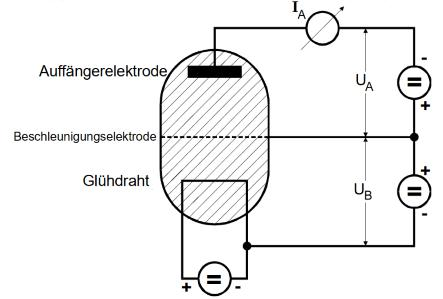
\includegraphics[width=\linewidth-70pt,height=\textheight-70pt,keepaspectratio]{content/images/apparatur.jpg}
\caption{Schematischer Aufbau einer Franck-Hertz-Apparatur \cite{V601}.}
\label{fig:apparat}
\end{figure}
\begin{figure}
\centering
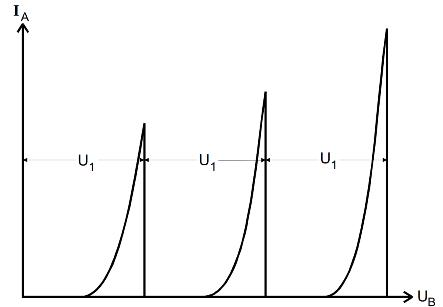
\includegraphics[width=\linewidth-70pt,height=\textheight-70pt,keepaspectratio]{content/images/I_theo.jpg}
\caption{Der an der Elektrode ankommende Strom $I$ in Abhängigkeit von der Beschleunigungsspannung $U_.B$ \cite{V601}.}
\label{fig:I_theo}
\end{figure}
\subsection{Das Kontaktpotential}
Um die Elektronenausbeute zu erhöhen wird die üblicherweise aus Wolfram bestehende Kathode mit einem Material niedrigerer Austrittsarbeit $\Phi_.G$ beschichtet. Für die Beschleunigerelektrode hingegen wird ein Material mit hoher Austrittsarbeit $\Phi_.B$ verwendet, um dort Elektronenaustritte zu verhindern.
Dadurch kommt es allerdings zum Kontaktpotential
\begin{equation}
K=\frac{1}{e_.0}\left(\Phi_.B-\Phi_.G\right)\text{,}\label{eq:kontakt}
\end{equation}
welches den Verlauf der Franck-Hertz-Kurve verschiebt. Für die effektive Beschleunigungsspannung gilt:
\[
U_.{B,eff}=U_.B-K
\]
Das Potentialgefälle zwischen $\Phi_.G$ und $\Phi_.B$ ist in Abbildung \ref{fig:kontakt} abgebildet.
\begin{figure}
\centering
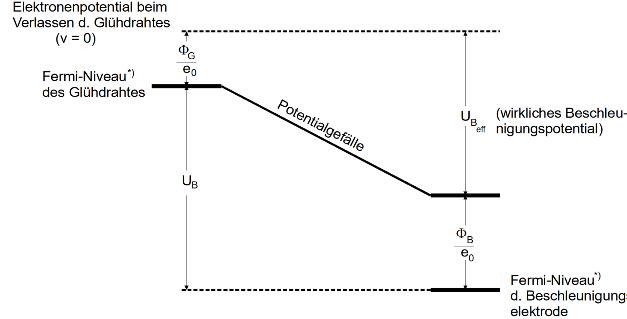
\includegraphics[width=\linewidth-50pt,height=\textheight-50pt,keepaspectratio]{content/images/kontaktpot.jpg}
\caption{Das Verhältnis zwischen dem Potential der Glühkathode $\Phi_.G$ und dem der Beschleunigerelektrode$\Phi_.B$ \cite{V601}.}
\label{fig:kontakt}
\end{figure}
\subsection{Die Energieverteilung der Elektronen}
Ein weiterer Faktor der zur Verschlechterung der Franck-Hertz-Kurve führt ist, dass die Energie der Elektronen in der Kathode der Fermi-Dirac-Verteilung in Abbildung \ref{fig:fermi} folgt und somit die austretenden Elektronen nicht alle dieselbe kinetische Energie besitzen. Das führt dazu, das einige hochenergetische Elektronen bereits die zur Anregung nötige Energie besitzen, bevor $U_.{B,eff}$ den nötigen Wert erreicht. Die Stromkurve wird dadurch nicht mehr beim Erreichen von $U_.1$ auf 0, sondern stetig auf ein mit jedem Peak wachsendes Minimum abfallen.
\begin{figure}
\centering
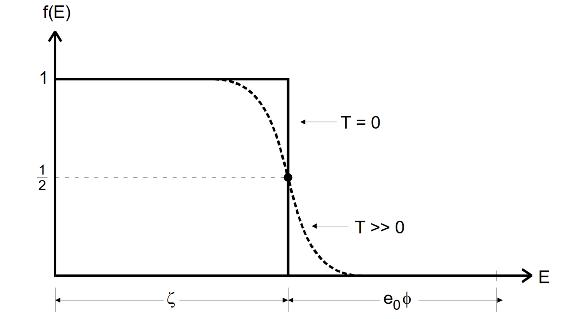
\includegraphics[width=\linewidth-70pt,height=\textheight-70pt,keepaspectratio]{content/images/fermi.jpg}
\caption{Verlauf der Fermi-Dirac-Verteilung am absoluten Nullpunkt und für wesentlich größere Temperaturen \cite{V504}.\label{fig:fermi}}
\end{figure}
\subsection{Der Dampfdruck}
Je höher der Druck des Hg-Gases im Inneren des Glaskolbens ist, desto häufiger stoßen die Elektronen mit Atomen zusammen. Der Weg den die Elektronen zurücklegen müssen, lässt sich deshalb durch die effektive Weglänge in Abhängigkeit von der Temperatur $T$ beschreiben als
\begin{equation}
\bar{w}[cm]=\frac{0,0029}{5,5\cdot10^7}\exp{\left(\frac{6867}{T}\right)}\text{.}\label{eq:w}
\end{equation}
Ist $T$ zu gering und somit der Druck zu groß, so stoßen sämtliche Elektronen bevor sie die Auffangelektrode erreichen und es wird kein Strom mehr gemessen. Ist der Druck hingegen zu gering, kommt es nur zu wenigen inelastischen Stößen und einige Elektronen erreichen genügend hohe Energien, um die Hg-Atome direkt in einen höheren Energiezustand als $E_.1$ anzuregen, sodass keine Franck-Hertz-Kurve mehr zu erkennen ist.
Um den optimalen Arbeitsbereich der Apparatur zu finden muss gelten $\bar{w}\ll a$, mit dem Abstand $a$ zwischen Kathode und Gitter.